\section{Choosing a generator}

Presently eleven alternative generators have been implemented in \textsc{MaGe}.
The actual generator to be used has to be set via the macro command

\begin{lstlisting}
 /MG/generator/select [PNNLiso] [RDMiso] [TUNLFEL] [G4gun] [decay0]
   [cosmicrays] [musun] [SPS] [neutronsGS] [wangneutrons] [sources4a]
   [AmBe] [MuonsFromFile] [GSS]
\end{lstlisting}

\textsc{G4Gun} is the default G4ParticleGun provided by Geant4.

\begin{table}[tp]
\caption{Summary table of the generators available in \mage}
\label{Table:generators}
\begin{center}
\begin{tabular}{|c c|}
\hline
Events to be generated & Generator \\
\hline
Double beta decay ($2\nu$ or $0\nu$) & decay0 \\
\hline
Radioactive contaminations & G4gun \\
 & PNNLiso \\
 & RDMiso \\
 & decay0 \\
 & SPS \\
\hline
Cosmic-ray muons & cosmicrays \\
 & musun \\
 & MuonsFromFile \\
\hline
Cosmogenic neutrons & neutronsGS (for LNGS) \\
 & wangneutrons \\
\hline
Neutrons from fission and ($\alpha$,n) & neutronsGS (for LNGS) \\ 
 & Sources4a \\
\hline
Neutrons (and $\gamma$-rays) from AmBe & AmBe \\
\hline
TUNFEL beam & TUNFEL \\
Surface Contamination & GSS \\
\hline
\end{tabular}
\end{center}
\end{table} 

\section{AmBe Generator}
%FixME owned by Alexis
The americium beryllium (AmBe) generator is a point source of neutrons and 
gammas. The AmBe neutron spectrum used comes from Figure 5 of Marsh,
Thomas, and Burke, "High resolution measurements of neturon
energy spectra from Am-Be and Am-B neutron sources", Nucl. Inst.
and Meth. A 366 (1995) 340-348. Gamma energies are taken from the $^{12}$C 
level structure, at
from http://www.nndc.bnl.gov/nudat2/getdataset.jsp?nucleus=12C.
Choice of gammas depending on neutron energy is taken from Figure 3 of 
Geiger et al., Nucl. Inst. and Meth. 131 (1975) 315.
 
  


\section{PNNL Radioactive Decay Chain Generator}

\subsection{General description}

 The PNNL radioactive decay chain generator consists of a set of G4 classes for
sampling charged particles (beta or alpha) and associated gammas arising from 
the decay of any radioisotopes in a user-{}specified radioactive decay chain.
Information returned by the generator is currently limited to the charged
particle type (beta+/-{} or alpha), charged particle energy, number of ``cascade"
gammas, and a list of gamma energies.  Currently the code is limited to linear
decay chains, i.e. multiple branch points in a decay chain yielding distinct
nuclear species are not (easily or naturally) supported.  (If only gammas are
of interest, however, a multiple-{}branch kludge is possible if the branches
merge in a common daughter.)  The generator code requires as input the gamma 
cascade branching fractions for each radioisotope in the decay chain (one
ascii-{}format file per radioisotope), and a master ``decay chain" ascii-{}format
file specifying the number of radioisotopes in the chain, the decay half-{}lives
for each isotope and the names of each isotope's cascade file.  The cascade
branching fractions can be calculated using the tool CrazyInput, written by 
J.E. Ellis and A. Valsan of PNNL.  As currently implemented, setup of the 
generator requires running CrazyInput once for each radioisotope in the decay 
chain of interest.  The ascii-{}format files output by CrazyInput are then
collected in a single directory and read by the generator upon initialization.
Terminology used in this paragraph is explained in more detail below.
 

 The main object/data structure in the generator is a DecayChain object, 
representing e.g. the Thorium decay chain (consisting of the radionuclides 
Th-{}232, Ra-{}228, Ac-{}228, ..., Pb-{}208). The DecayChain's primary 
responsibilities are to serve as a container for radioisotopes, embodied in 
Radioisotope objects, to calculate the relative decay probability for each 
member isotope of the chain based upon the grow-{}in age of the source, and to 
sample appropriately from each Radioisotope object's decay.  Each Radioisotope
object can decay by either beta(+/-{}) or alpha emission, accompanied by the 
emission of one or more ``cascade" gammas from the daughter nucleus.  A cascade
is defined as a single decay scheme of a single radioisotope: For example, 
beta decay to a given excited state in the daughter nucleus, followed by 
emission of N gammas of energy E1, E2, ..., EN.  (Currently no time 
information is associated with the cascade gammas, which are assumed emitted 
in coincidence.) In general, a single radioisotope can decay via multiple 
cascade schemes.  Within the generator framework, each Radioisotope object 
thus contains one or more Cascade objects, each of which contains all of the 
information necessary for setting up and sampling from e.g. a beta decay 
energy distribution specific to that cascade decay scheme.  Each Cascade 
object also contains a list of coincident gammas associated with the cascade.
Each Radioisotope object stores a list of branching fractions for the set
of cascade it contains, and its primary responsibility is to sample from
the set of cascades associated with it when interrogated by the DecayChain
object for the current event.  In turn, a particular Cascade object ``knows"
how to sample from the beta distribution associated with it.  (Mono-{}energetic
alphas can also be associated with a cascade scheme.)  The logical structure 
of the generator is thus a nesting of data structures: a DecayChain object 
contains one or more Radioisotope objects, which in turn contain one or more 
Cascade objects.  These objects are described in the classes 
MGGeneratorPNNLDecayChain, MGGeneratorPNNLRadioisotope, and 
MGGeneratorPNNLCascade, respectively.
 

 The three main tasks of the PNNL generator are as follows: (1) Upon 
initialization, read a set of user-{}supplied files defining the decay chain and
specifying the set of cascade schemes appropriate to each radioisotope in the 
chain.  (2) Determine the relative activities (via standard Bateman equation 
calculations) of each radioisotope in the decay chain, given a user-{}supplied
list of the half-{}lives of each isotope in the chain and the grow-{}in time, T,
appropriate for the material.  It is assumed that T=0 corresponds to a material
consisting entirely of the isotope at the head of the chain.  (3) For event
sampling, select the next radioisotope to decay (based upon relative activities
of each isotope in the chain), and for that isotope, select a given cascade
decay scheme (based on cascade branching fractions determined by the CrazyInput
tool).  The energy of the decay beta (or the single energy of an alpha) is 
then sampled from an appropriate distribution and the list of corresponding
decay gammas (if any) retrieved from the appropriate Cascade object.  The 
generator returns a CascadeEvent object to the calling routine (e.g. the 
GeneratePrimaries member function of the PrimaryGeneratorAction class) for
the current event, and all information (e.g. particle types and energies) 
relevant to the radioactive decay can be extracted from this simple data 
structure in preparation for adding particles to the tracking stack.
 

\subsection{Using the generator}

\subsubsection{Setup}

 Setting up the generator currently requires (1) creating a set of ascii-{}format 
files (one for each radioisotope in the decay chain of interest) using the 
CrazyInput cascade branching-{}fraction calculation tool; (2) collecting these 
files in a convenient sub-{}directory; and (3) creating a master ``decay chain 
file" to describe to the generator the number of isotopes in the chain, the
half-{}life of each isotope, and the files listing the cascade branching
fractions for each isotope.
 

 An example cascade branching-{}fraction file for Tl-{}208 is displayed below.
 

\begin{lstlisting}
 208.0   81.0   10
 0.49499E+00    1.79626   1   1   2
  0.58319  2.61453
 0.23966E+00    1.28556   1   1   3
  0.51077  0.58319  2.61453
 0.12545E+00    1.51889   1   1   2
  0.86056  2.61453
 0.96121E-01    1.51889   1   1   3
  0.27736  0.58319  2.61453
 0.18924E-01    1.03304   1   1   3
  0.76313  0.58319  2.61453
 0.11496E-01    1.03304   1   1   4
  0.25261  0.51077  0.58319  2.61453
 0.39991E-02    1.07420   1   1   4
  0.21140  0.51077  0.58319  2.61453
 0.37982E-02    1.28556   1   1   2
  1.09390  2.61453
 0.31466E-02    1.28556   1   1   3
  0.23336  0.86056  2.61453
 0.24109E-02    1.28556   1   1   0
\end{lstlisting}

 The first line of the file lists A, Z, and the number of cascades contained
in the file.  Each cascade consists of two lines of input.  The first
line lists, in order, the branching fraction for the cascade, the endpoint
energy for the beta decay spectrum (or the alpha-{}particle energy) in MeV, the 
charged particle type (0 for alpha, 1 for beta, 2 for positron), the angular
momentum change, ``delta(L)" (in units of hbar), suffered by the nucleus in 
the decay, and the number of gammas associated with the de-{}excitation cascade 
emitted by the daughter nucleus.  The second line of the cascade description
lists the energies of the cascade gammas (MeV).  In the example file, 10 
cascade decay-{}schemes for Tl-{}208 are listed.  Reading from the second and 
third lines of the file, the first decay scheme is beta decay with an endpoint
energy of 1.79626 MeV and delta(L) of 1.  The beta is accompanied by 2 cascade
gammas of energy 0.58319 and 2.61453 MeV, respectively.
 

 In general, for a decay chain consisting of N radioisotopes, each radioisotope
must be described by a cascade branching fraction file in the format shown
above.  In addition to these files, an ascii-{}format ``decay chain file" must
be supplied to inform the generator of the general decay chain structure.  An
example file for the Th-{}232 decay chain is exhibited below.
 

\begin{lstlisting}
10
 1  Th-232   1.41e10  y  dat/cascades_232Th.dat
 2  Ra-228   5.75     y  dat/cascades_228Ra.dat
 3  Ac-228   6.15     h  dat/cascades_228Ac.dat
 4  Th-228   1.910    y  dat/cascades_228Th.dat
 5  Ra-224   3.64     d  dat/cascades_224Ra.dat
 6  Rn-220  55.0      s  dat/cascades_220Rn.dat
 7  Po-216   0.15     s  dat/cascades_216Po.dat
 8  Pb-212  10.64     h  dat/cascades_212Pb.dat
 9  Bi-212  60.6      m  dat/cascades_212Bi.dat
10  Tl-208   3.05     m  dat/cascades_208Tl.dat
\end{lstlisting}

 The first line in the decay chain file lists the number of radioisotopes in the
chain (10 in this example).  Each radioisotope is described in a single line.
The first entry in a radioisotope line is an (arbitrary) integer index which 
is not used by the code but may be useful to the user.  The second entry is
a string isotope label, used only in diagnostic messages output by the 
generator.  The third and fourth entries specify the decay half-{}life and the
units of the entry: (y,d,h,m,s) for (year, day, hour, minute, and second)
respectively.  The final entry lists the name and path of the cascade branching
fraction file for the radioisotope, relative to the directory in which the
G4 code is to be run.  (This ``main" directory will contain e.g. a macro file
containing G4 messenger commands, as well as the master decay chain file.)
 

 In summary, note that the user must (currently) construct the master decay 
chain file by hand.  The cascade branching-{}fraction files, one for each 
radioisotope, are generated by running the CrazyInput tool.  Once these files
are available and the decay chain file has been constructed, generator setup 
for the particular decay chain of interest is complete.
 

\subsubsection{Initializing the generator}

 Once the required set of input files has been prepared, initialization of the 
generator is controlled by two messenger commands in a G4 macro file, as
demonstrated in the example which follows:
 

\begin{lstlisting}
 /generator/PNNL/init Th232_DecayChain.dat
 /generator/PNNL/setSourceAge 5.0
\end{lstlisting}

 In this example, the command ``/generator/PNNL/init Th232\_DecayChain.dat"
informs the primary event generator code that the PNNL radioactive decay
chain generator will be used in the G4 run, and initializes the generator with
the name of the decay chain control file.  Typically this control file will
reside in the same directory as the G4 macro file controlling the batch run.
The command ``/generator/PNNL/setSourceAge 5.0" sets the source grow-{}in age
to 5.0 years in this example.  Recall that the relative activities of each
radioisotope in the decay chain are calculated using the Bateman equations,
with the assumption that time T=0 corresponds to a source consisting solely
of the material at the head of the decay chain (Th-{}232 in this example.)  If
the setSourceAge messenger command is not issued, the default value for the
grow-in age is 0.  In this case, only radioactive decays from the isotope at 
the head of the chain are sampled by the generator.
 

 In summary, the general messenger command structure is as follows:
 

\begin{lstlisting}
 /generator/PNNL/init [master decay chain filename]
 /generator/PNNL/setSourceAge [source grow-in age in years]
\end{lstlisting}

\section{Decay0 Generator}

\textsc{Decay0} is a primary generator developed by Vladimir I. Tretyak. 
It can generate two-neutrinos double beta decay events, and neutrinoless double beta decay 
according to a large number of theoretical models and background events from the most common 
$\gamma$/$\beta$ sources (low-probability transitions are included); it can also produce 
generic $\beta$ spectra and mono-energetic particles. The most recent version of 
\textsc{Decay0} accounts for the angular correlation between $\gamma$-rays emitted in 
$^{60}$Co and in the two-neutrino double beta decay of $^{76}$Ge to the $0^{+}_{1}$ 
excited state of $^{76}$Se (1122~keV).\\ 
\textsc{Decay0} accounts for the kinematic of the final state (i.e. momenta of all 
the particles) and for the time, which is relevant for chains or delayed 
de-excitation (e.g. $^{137}$Cs+$^{137m}$Ba). It is a \texttt{Fortran} standalone 
program and the MG generator class (MGDecay0Interface.hh) reads from the ASCII files 
dumped by it: the user must take care that the file contains enough 
events for the Geant4 simulation (otherwise the program will give an 
exception). \\
\textsc{decay0} is not a part of \mage, but the \texttt{Fortran} source code for 
the most recent version is included in the CVS repository, in the directory \texttt{GETools}. 
It must be compiled and linked with the CERN Fortran libraries. \\
%
The \textsc{Decay0} generator is instantiated with the macro command:
%
\begin{lstlisting}
 /MG/generator/select decay0
\end{lstlisting}
%
and the file to be read is set with the command  
%
\begin{lstlisting}
 /MG/generator/decay0/filename myfile.txt
\end{lstlisting}
%
The file name must be set before the \texttt{/run/beamOn}.
%
\section{Cosmic rays generator}\label{Chapter:cosmic_rays}
%FixME owned by Luciano
It is used to generate high-energy muons with the characteristic spectrum 
of cosmic rays in underground sites. 
The primary position is sampled from a disk of radius $r$ (default = 8 m) placed 
at the height $h$ (default = 8.1 m). Both these values can be changed via messenger.\\ 
The energy spectrum is sampled using the analytical parametrization of  
Lipari and Stanev~\cite{Lipari:1997}, which applies to rock depths 
between 1 km w.e. and 10 km w.e. The spectral index of the muon spectrum can be 
3.7 (standard), 2.7 (Prompt sources, e.g. charm decay) or 2.0 (Exotic sources). The 
defaults are 3400 m w.e. (Gran Sasso depth) and 3.7 respectively. \\
The angular spectrum is sampled according to the measurements performed at Gran Sasso 
by the MACRO experiment. The MACRO data are loaded from an ASCII file in the 
directory \texttt{\$MGGENERATORDATA}. If the file is not present, the distribution is 
sampled according to $\cos^{-1}\theta$, as described in Ref.~\cite{Lipari:1997}. 
In the latter case, a warning message is printed on the screen.

The cosmic ray generator is instantiated with the macro command:

\begin{lstlisting}
 /MG/generator/select cosmicrays
\end{lstlisting}

The commands to change the parameters of the generator are:
\begin{lstlisting}
 /MG/generator/cosmicray/radius radius [unit]
 /MG/generator/cosmicray/height radius [unit]
 /MG/generator/cosmicray/depth  depth [unit]
 /MG/generator/cosmicray/index index
\end{lstlisting}

for radius, height, depth (with unit) and spectral index respectively.
 
\section{The muons from file generator}\label{Chapter:muons_from_file}

This generator was developed, to allow the user to select muons from a file, instead 
of using the cosmic rays generator, that was introduced in the previous chapter \ref{Chapter:cosmic_rays}.
It reads the starting position, the direction and the energy of the muon from a file with a structure like:
\begin{lstlisting}
 pos(x) pos(y) pos(z)  dir(x) dir(y) dir(z)  energy
\end{lstlisting}
with the three dimensions of the starting position \textit{pos(x,y,z)}, the three elements of the direction
vector \textit{dir(x,y,z)} and the \textit{energy} of the muon. It was mainly used to simulate a set of muons, 
that were identified as dangerous, i.e. during their simulation, an energy deposition around 2 MeV in the germanium crystals
was registered. An example of a small file is given in tabular \ref{Tab:muon_example}.
\begin{table}[tp]
\caption{Example table of some dangerous muons for \mage. The header must not be included into the file.}
\label{Table:generators}
\begin{center}
\begin{tabular}{|c|c|c|c|c|c|c|}
\hline
 pos(x) & pos(y) &  pos(z) & dir(x) & dir(y) & dir(z) & energy \\ \hline \hline
1199.75 & 69.6281 & 810 & -0.836506 & -0.0649792 & -0.544091 & 370888 \\
200.717 & 541.989 & 810 & -0.301985 & -0.469251 & -0.829825 & 914548 \\
305.095 & -292.536 & 810 & -0.355895 & 0.34182 & -0.869769 & 1.31997e+06 \\
-1476 & -727.268 & 810 & 0.812514 & 0.390033 & -0.433238 & 570688 \\
-474.305 & -731.501 & 810 & 0.421681 & 0.602593 & -0.677545 & 213939 \\ \hline
\end{tabular}
\end{center}
\end{table}

The muons from file generator is initiated with the macro command:

\begin{lstlisting}
 /MG/generator/select MuonsFromFile
\end{lstlisting}

The commands to change the parameters of the generator are:
\begin{lstlisting}
/MG/generator/MuonsFromFile/filename file
\end{lstlisting}

to change the name of the file, from which the muons are read in. The files have to be stored 
into the MGGENERATORDATA folder. 




\section{MUSUN Generator}
\textsc{MUSUN} is a primary generator developed by Vitaly Kudryavtsev and described 
in \cite{Kudryavtsev:1997}. It is \texttt{Fortran}-based and it is able to track 
high-energy muons through large thicknesses of rock, to obtain the muon spectrum (energy and 
direction) inside an underground Laboratory. It can also take into account 
the depth profile of the specific Laboratory, if available, in order to 
reproduce the possible asymmetries in the azimuth distribution. The \mage  
generator is istantiated with the command:
\begin{lstlisting}
 /MG/generator/select musun
\end{lstlisting}
%
It reads the event kinematic parameters (energy and direction) of 
the primary muon from an ASCII file, whose name (and path, if it is not 
in the current directory) has to be provided using the macro command 
%
\begin{lstlisting}
 /MG/generator/musun/filename myfile.txt
\end{lstlisting}
%
The primary position is sampled from a disk of radius $r$ (default = 8 m) placed 
at the height $h$ (default = 8.1 m). Both these values can be changed via messenger, 
using the same commands described in the previous section for the CosmicRay 
generator, i.e. 
%
\begin{lstlisting}
 /MG/generator/cosmicray/radius radius [unit]
 /MG/generator/cosmicray/height height [unit]
\end{lstlisting}
  
\section{NeutronsGS generator}
This generator produces neutrons induced by natural radioactivity and interactions of cosmic-ray 
muons in the rock. Energy is sampled according to the spectrum at Gran Sasso reported 
in Ref.~\cite{Wulandari:2004}. The generator is instantiated with the command 
 
\begin{lstlisting}
 /MG/generator/select neutronsGS
\end{lstlisting}

The data are read from ASCII files, that are looked for in the directory 
\texttt{\$MGGENERATORDATA}. 
It is possible to generate either the low-energy component from 
fission and ($\alpha$,n) from the rock or the high-energy component induced 
by muon interactions in the rock. The latter is the default. The spectrum to 
be generated can be selected via messenger:
\begin{lstlisting}
 /MG/generator/neutrons/fission [true] [false]
\end{lstlisting}
If the value \texttt{true} is assigned, the low-energy component produced by natural 
radioactivity in the rock is considered.
The fission/($\alpha$,n) neutrons are considered to be isotropic, while the 
angular distribution of the high-energy component is sampled according to 
\cite{Wulandari:2004}. 
The position of the primary tracks is sampled from the 
upper surface, the lower surface or the lateral surface of a cylinder; it 
can be set with the command:
\begin{lstlisting}
 /MG/generator/neutrons/direction [roof] [floor] [walls]
\end{lstlisting}
The dimensions of the cylinder are 8.0~m radius and 8.0~m height. The defaults 
can be changed with the commands
\begin{lstlisting}
 /MG/generator/neutrons/radius radius [unit]
 /MG/generator/neutrons/height height [unit]
\end{lstlisting}
%

\section{Sources-4A Generator}
\textsc{Sources-4A} is a \texttt{Fortran}-based generator of neutrons produced 
in a given material by fission and by ($\alpha$,n) reactions on light elements. 
It has been developed by the LANL; a large number of cross section tables for 
various elements has been recently added in the context of the ILIAS 
EU work. The code calculates the energy spectrum of the emitted neutrons; 
the angular distribution is assumed to be isotropic. The explicit 
tracking of the neutron (out of its source, for instance) is not done 
by \textsc{Sources-4A} but has to be performed using \mage\ and \geant.\\ 
The output from \textsc{Sources-4A} is the absolute energy distribution of neutrons; 
the total production rate is expressed in \mbox{neutrons cm$^{-3}$ s$^{-1}$}. The name of the 
output file from \textsc{Sources-4A} containing the absolute energy spectrum is \texttt{tape7}. 
The \mage \ generator is istantiated with the command
 
\begin{lstlisting}
 /MG/generator/select sources4a
\end{lstlisting}
In the default case, the data file to be read is called \texttt{tape7} and it is 
looked for in the current directory. The file name can be alternatively specified 
(with its path) using the command 
\begin{lstlisting}
 /MG/generator/sources4a/filename myfile.txt
\end{lstlisting}
The generator also works if the normalized energy spectrum (called 
\texttt{tape8} in the default case) is used.\\ 
The only limitation of the generator is that the lower egde of the lowest-energy 
bin must be zero. The generator does not take care of the position sampling of the 
neutron; in most case, it will be appropriate to use the uniform position sampling in 
a given volume, which is described in Sect.~\ref{Section:positionsampling}. 

\section{General Particle Source}\label{sec:GPS}
{\em Note:  The GPS has many, many options, not all of which are covered in this
manual.  For a complete list, look at the \geant \ source code.  Once you give
that up, look at the much more accessible GPS user's manual at
\hbox{http://reat.space.qinetiq.com/gps/}.  It explains everything and also contains many example
macros.} 

The \geant \ General Particle Source (GPS) was designed to supplant the G4Gun as a
general source for any particles you might want to use.  It also allows for
position sampling, angular and energy distributions, and multiple sources.  To use the GPS, the messenger command is
%
\begin{lstlisting}
 /MG/generator/select SPS
\end{lstlisting}
The GPS can sample from several types of planes(circle, annulus, ellipsoid,
square, rectangle) and surfaces/volumes(sphere, ellipsoid, cylinder,
parallepiped).   Messenger commands set the sizes, positions, and attributes of
the original positions.  Some examples are
%
\begin{lstlisting}
 /gps/position 1.0 2.0 2.5 cm
 /gps/pos/type Plane
 /gps/pos/shape annulus
 /gps/pos/radius 5.0 cm
 /gps/pos/inner_radius 3.0 cm
\end{lstlisting}
%
The angular and energy distributions can also be customized.  The choices for
angular distributions are isotropic,
cosine-law, or user-defined.  You can also choose parallel beam or a diverging
accelerator beam.  For energy distributions, you can choose from mono-energetic,
linear, exponential, power-law, gaussian, bremsstrahlung, black body, and cosmic
diffuse gamma ray.  Some example messenger commands utilizing these(taken from
Example 13 in the GPS user's manual,
\hbox{http://reat.space.qinetiq.com/gps/examples/examples.htm}):
%
\begin{lstlisting}
 /gps/ang/type cos
 /gps/ene/type Exp
 /gps/ene/min 2. MeV
 /gps/ene/max 10. MeV
 /gps/ene/ezero 6.
\end{lstlisting}
%
The GPS uses the \geant \ native radioacative decay module (RDM).  To set up an
ion and set limits on it's decay, 
\begin{lstlisting}
 /gps/ion <Atomic Number> <Mass Number> <Ionic Charge> <Excitation Energy>
 /grdm/nucleusLimits <Amin> <Amax> <Zmin> <Zmax>
\end{lstlisting}

To set up
a radioactive ion, say $^{238}$U, and let it decay to $^{222}$Rn, the messenger
commands would be
%
\begin{lstlisting}
 /gps/particle ion
 /gps/ion 92 238 0 0
 /gps/energy 1e-20 eV
 /grdm/nucleusLimits 222 238 86 92 
\end{lstlisting}
%
\noindent

\section{Position sampling} \label{Section:positionsampling}
Only a few of the generators described above take care of sampling the initial position of 
the primary particle. Notably, they are: TUNFEL, MUSUN, CosmicRays, NeutronsGS,
and \hbox{SPS}/\hbox{GPS}(General Particle Source).
%%FIXME is this accurate?  RAJ 21Feb2007
For 
all the others, the source is considered to be a fixed point.
The default is the origin of the coordinate system, but it can be set (for any generator) 
with the macro command
\begin{lstlisting} 
 /MG/generator/position coordinates [unit]
\end{lstlisting}
The command has no effect on the TUNFEL, MUSUN, CosmicRays and NeutronsGS generators, that 
internally overwrite the position of the primary particle. For the G4gun generator only, the 
command 
\begin{lstlisting} 
 /gun/position coordinates [unit]
\end{lstlisting}
can also be used.  The General Particle Source (GPS) has all of the features of
the G4gun, but also much more in the way of position sampling and angular/energy
biasing.\\
%
\subsection{Uniform sampling} 
For some applications (e.g. simulation of internal contamination) it 
is useful to sample the position of the primary event uniformly within a given 
physical volume or a given skin surface. 
The \mage \ package includes an algorithm for this purpose. 
The confinement level (noconfined, volume, surface) is set with the command: 
 
\begin{lstlisting}
 /MG/generator/confine   [noconfined] [volume] [surface] [volumelist]
\end{lstlisting}

The default is \texttt{noconfined} (e.g. primary generated in a fixed position). 
If the confinement level is set to \texttt{volume}, the physical volume 
has to be set with the command 
 
\begin{lstlisting}
 /MG/generator/volume volumename
\end{lstlisting}

\noindent where \texttt{volumename} is the name of an existing physical volume. This command has 
to be called after /run/initialize. If the volume name is not unique (e.g. replicas exist), 
the copy numbered ``0" will be taken into account.  The surface confinement
level has not been implemented in this context, but an alternate method exists
and is covered in Section \ref{sec:surfacesampling}. \\

\subsubsection{Confinement in geometrical volumes or surfaces}
It is also possible to sample the position of the primary event uniformly in a geometrical 
volume (e.g. a spherical shell, or a cylinder) or a geometrical surface (e.g. a disk, or a sphere). 
Although this functionality is already provided by the General Particle Source generator 
(see sect.~\ref{sec:GPS}), the General Particle Source treats also direction sampling and it is 
not possible to use the tools described in Sect.~\ref{sec:direction}, as the sampling of the 
direction of the primary particle within a given angle from a target position. The position sampling 
over a geometrical volume/surface, as provided by \mage, can be coupled with the tools for 
direction sampling.

The confinement level is set with the command 
\begin{lstlisting}
 /MG/generator/confine   [noconfined] [geometricalvolume] [geometricalsurface] 
\end{lstlisting}

The shape for the geometrical volume/surface can be set with the commands
\begin{lstlisting}
 /MG/generator/geomSampling/volume/name [Sphere] [Cylinder] 
 /MG/generator/geomSampling/surface/name [Sphere] [Cylinder] [Disk] 
\end{lstlisting}
The geometrical volume/surface defined in this way may include one or more \mage\ physical 
volumes. The center of the target volume/surface is given as
\begin{lstlisting}
/MG/generator/geomSampling/volume/center x y z [cm] 
/MG/generator/geomSampling/surface/center x y z [cm]
\end{lstlisting}
The default position is the origin of the reference frame. Dimensions of volumes are given using 
the messenger:
\begin{lstlisting}
/MG/generator/geomSampling/volume/innerSphereRadius x [cm]
/MG/generator/geomSampling/volume/outerSphereRadius x [cm]

/MG/generator/geomSampling/surface/sphereRadius x [cm]

/MG/generator/geomSampling/surface/innerDiskRadius x [cm]
/MG/generator/geomSampling/surface/outerDiskRadius x [cm]

/MG/generator/geomSampling/surface/innerCylinderRadius x [cm]
/MG/generator/geomSampling/surface/outerCylinderRadius x [cm]
/MG/generator/geomSampling/surface/cylinderHeight x [cm]

/MG/generator/geomSampling/volume/innerCylinderRadius x [cm]
/MG/generator/geomSampling/volume/outerCylinderRadius x [cm]
/MG/generator/geomSampling/volume/cylinderHeight x [cm]
\end{lstlisting}
Default values for the inner radii is 0; all other dimensions (outer radius, and possibly 
heights) must be specified before the \texttt{/run/beamOn}.

\subsection{Surface sampling} 
\label{sec:surfacesampling}
%FixME owned by Jason, Rob, Mike, and Reyco
\geant \ cannot effectively sample complex surfaces(in particular, boolean solids
composed of unions of elementary solids).  The Generic Surface Sampler (GSS) was
created to get around this.  Randomly sampled points from surfaces in
\mage \ can be acquired by using the GSS.  These points are stored as x, y, and z
coordinates in a \rootv tree (GSSTree),  within a \rootv file.  The actual
physics simulation
is then run, using this file as a source for primary vertices corresponding to
the surface of interest.  Note that this involves running \mage \ twice, first to
get the position points, and then for the physics.  The GSS can sample one or many different volumes within a geometry at once.  The macro commands to use the GSS and to name the GSS \rootv file are

\begin{lstlisting}
 /MG/eventaction/rootschema GSS
 /MG/eventaction/rootfilename GSSfilename.root
\end{lstlisting}

The names of the physical volumes that are to be sampled are given to the GSS by
messenger commands.  For example, the following messenger commands would add
three volumes; two crystals in the \majorana reference design and the outer
cryostat.

\begin{lstlisting}
/MG/io/gss/addVolume InnerCryostatPhysical
/MG/io/gss/addVolume Crystal1CrystalColumn2
/MG/io/gss/addVolume Crystal0CrystalColumn13
\end{lstlisting}
\noindent For a given run of the GSS, all of the sampled volumes will have the
same surface density of sampled points.  Alternatively, you can of course sample
individual volumes separately.

The algorithm for GSS requires the radius and center (centre) of a sphere that
completely envelops all of the volumes to sample.  There are two methods to do
this.  Messenger commands can set these values directly:

\begin{lstlisting}
 /MG/generator/gss/origin x y z
 /MG/generator/gss/boundingR R
\end{lstlisting}

\noindent where x, y, z, and R must of course have recognized units of length.  If all of
the volumes to be sampled are contained within some kind of holding container
(like an array of crystals in a cryostat), or if there is only one volume to be
sampled, then there is an easier way to handle the origin and radius.  The
messenger command

\begin{lstlisting}
 /MG/generator/gss/boundvol EncompassingPhysicalVolume
\end{lstlisting}

\noindent will ensure that the radius and origin are properly set.  Note,
``EncompassingPhysicalVolume" is the name of the physical volume that contains
all of the volumes to be sampled, and it need not be sampled itself.

\begin{figure}[h]
\begin{center}
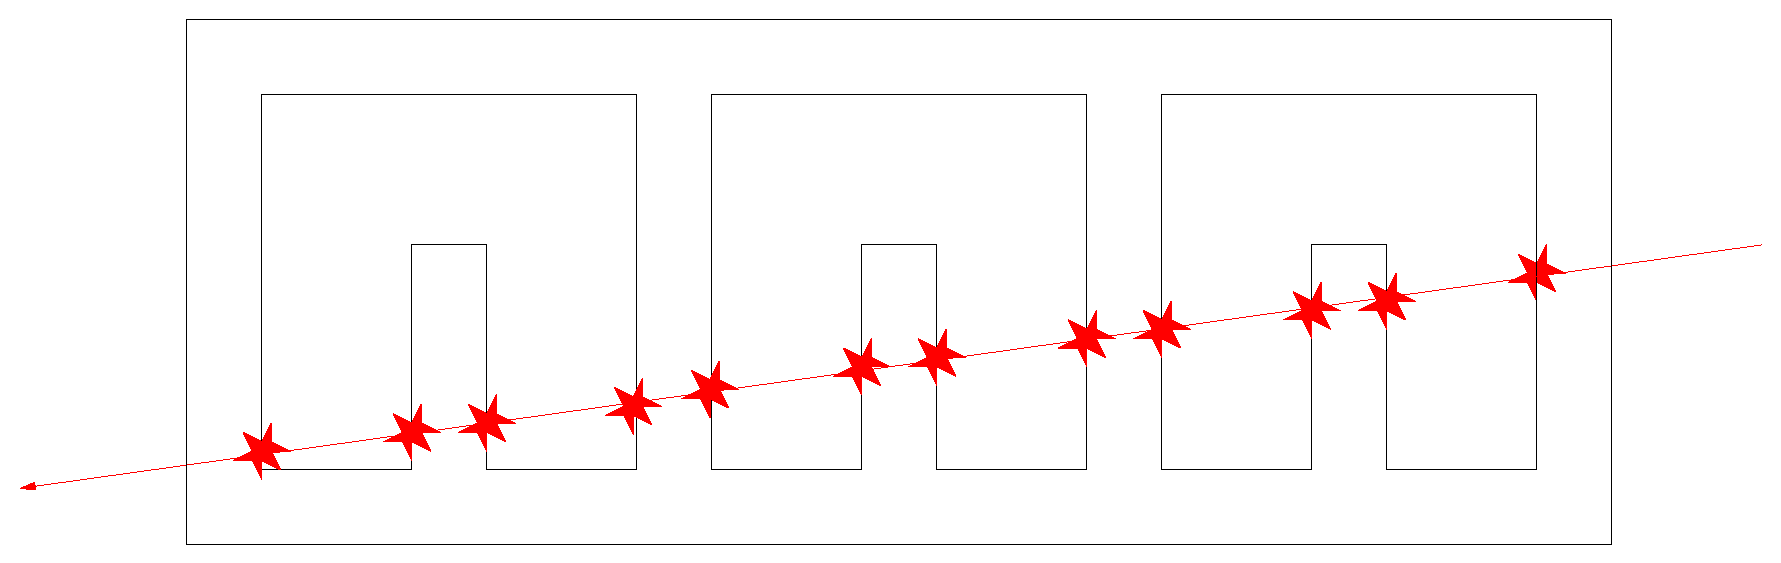
\includegraphics[width=0.6\textwidth]{Intersections}
\caption{Cartoon showing intersections of a geantino with sampled surfaces for
the GSS}
\label{fig:intersections}
\end{center}
\end{figure} 

The algorithm also requires the maximum number of possible intersections that a
line would make with the sampled volumes.  For example, Figure
\ref{fig:intersections} shows three semi-coax germanium crystals in an
enclosure.  For sampling the three crystals, the maximum number of intersections
a line would make with a sampled surface is 12.  If we were to also sample the enclosure, the
number would be 14.  To set the number of intersections, the messenger command
is

\begin{lstlisting}
 /MG/io/gss/setMaxIntersections aNumber
\end{lstlisting}

\noindent \mage \ will throw a warning if you pick a number that's too low.  Some
quick words about the efficiency of the GSS: setting the maximum number of
intersections too high will cause the GSS to unnecessarily throw away more
events, requiring a larger number of initial events to achieve the desired
number of points.  For a given number of initial events, the number of achieved
random points will vary depending on the geometry of the sampled volumes.
Sampling a sphere or pseudo-spherical assembly would be quite efficient, whereas sampling a long, thin pole would not be.

Once the desired surface points have been gathered by the GSS into a \rootv
file, it is a simple matter to use them for a physics simulation.  To read the
positions from a file, the messenger command is 

\begin{lstlisting}
 /MG/generator/gsspositionsfile GSSfilename.root
\end{lstlisting}

\noindent The GSS \rootv files will have some number of position points.  There is
an option to start at a point that is not the first one,

\begin{lstlisting}
 /MG/generator/gsseventnumber aNumber
\end{lstlisting}

\noindent but the default is to start at the beginning of the file.  If you add
more than one file, they will be chained together.


\section{Direction sampling} \label{sec:direction}
All generators but  \textsc{G4gun} sample the direction of primary particles, isotropically or 
according to specific distributions. \\

If \textsc{G4gun} is used, primary particles are shot along a given direction, 
that can be set with the macro command 
\begin{lstlisting}
 /gun/direction dx dy dz
\end{lstlisting}
It is not necessary that the components $(dx,dy,dz)$ are normalized. 
For instance, the command to generate particles directed in the negative direction 
of the z-axis is /gun/direction 0 0 $-$1. \\

Alternatively, it is possible to generate particles with direction sampled isotropically 
from a cone with given direction and given opening angle. The command to activate this 
option, which works only for the \textsc{G4Gun} generator, is
\begin{lstlisting}
 /MG/generator/g4gun/cone_on true [true] [false]
\end{lstlisting}
By default, the \texttt{cone\_on} option is set to \texttt{false} (i.e. pencil beam). 
The direction of the cone axis can be specified with the command
\begin{lstlisting}
 /MG/generator/g4gun/coneDirection dx dy dz
\end{lstlisting}
The default direction is along the positive z-axis. Similarly, the opening angle of the cone is 
set with the command
\begin{lstlisting}
 /MG/generator/g4gun/thetaDelta angle [rad/deg]
\end{lstlisting}
The default angle is 180~degrees. In this case, the direction of the primary particles is sampled 
isotropically in all the space, irrespectively of the specified direction.\\

In some applications, in order to save CPU time and optimize \mage \ performaces, it is useful to 
generate primary particles only towards the detector region. \mage \ has the
capability of sampling the direction of the primary particles only in the
direction of a given point.
This option is activated with the macro command
\begin{lstlisting}
 /MG/generator/g4gun/centric_effect_on [true] [false]
\end{lstlisting}
and the target coordinates are set using the command
\begin{lstlisting}
/MG/generator/g4gun/detector_center_position coordinates [unit]
\end{lstlisting}
Anyway, often one is not interest in a dimensionless target point, but rather in a target volume surrounding that 
point. This is necessary for instance to take into account for the extension of the real volumes and/or for changing in the 
particles direction along its propagation. There are two ways of specifying the extension of the target region 
around target point: 
\begin{enumerate}
\item the target volume is a box (default). The coordinates of the box are given with the command 
/MG/generator/g4gun/detector\_center\_position, while its dimensions along the x-, y- and z-axis are set with 
\begin{lstlisting}
/MG/generator/g4gun/detector_position_smear dimension [unit]
\end{lstlisting}
\item the direction is sampled within a cone pointing towards the target point. This option is activated 
with the command 
\begin{lstlisting}
/MG/generator/g4gun/centric_effect_cone [true] [false]
\end{lstlisting}
while the opening angle of the cone is specified by the macro command
\begin{lstlisting}
/MG/generator/g4gun/opening_angle angle [unit]
\end{lstlisting}
In this case, the direction of the cone axis depends on the initial position of the track, and it is internally 
re-calculated event-by-event.
\end{enumerate}    

\section{Energy sampling} \label{sec:energysampling}
All generators but  \textsc{G4gun} sample the energy of primary particles (e.g. cosmic ray muons, 
\textsc{Decay0}, etc.) according to their specific spectra. \\

If \textsc{G4gun} is used, primary particles are shot with a fixed kinetic energy, 
that can be set with the macro command 
\begin{lstlisting}
 /gun/energy energy [unit]
\end{lstlisting}
For instance, the command to generate 1-MeV particles is 
/gun/energy 1 MeV \\

Alternatively, it is possible to generate particles with energy spectrum sampled according 
to an histogram stored on a local file. This can be useful to generate energy spectra that 
are not provided by \textsc{Geant4}, as for instance $\beta$ spectra from forbidden transitions 
(e.g. $^{39}$Ar). In fact \textsc{Geant4} samples $\beta$ spectra according to the Fermi function, 
which is appropriate for allowed $\beta$-transitions only.
The command to activate this 
option, which works only for the \textsc{G4Gun} generator, is
\begin{lstlisting}
 /MG/generator/g4gun/spectrum_from_file [true] [false]
\end{lstlisting}
By default, the \texttt{spectrum\_from\_file} option is set to \texttt{false} (i.e. mono-energetic 
beam). \\
\emph{Notice} that energy sampling activated with the \texttt{spectrum\_from\_file} can be coupled with 
the direction sampling described in Sect~\ref{sec:direction} and the position sampling described in 
Sect.~\ref{Section:positionsampling}. For instance, it is possible to generate with \textsc{G4gun} 
primary particles emitted with a given energy spectrum (read from file), with direction in a given cone 
and with initial position distributed in a given volume. \\
% 
The file name containing the spectrum can be specified with the command
\begin{lstlisting}
 /MG/generator/g4gun/spectrum_filename [filename]
\end{lstlisting}
The information is taken into accouunt only if the flag from \texttt{spectrum\_from\_file} is set to 
\texttt{true} before the \texttt{/run/beamOn}. The program looks for the data file first in the current 
directory, and then in the directory pointed by the environment variable \texttt{MGGENERATORDATA}. Notice 
that \textsc{MaGe} will exit with an error code if one tries to run the \texttt{spectrum\_from\_file} 
option without having specified the file name and/or the data file is not found. 
The data file should have two column showing: 
\begin{lstlisting}
 energy (keV)  pdf of energy distribution (a.u.)
\end{lstlisting}

The energy spectrum does not need to be normalized, as it is re-normalized internally at the initialization 
time. The energy provided in the file should be the left edge of each bin. For the last bin, it is assumed 
that its width is equal to the width of last-but-one bin. \\

\nolinkurl{Warning}: the sampler DOES NOT interpolate inter-bin ranges. It means that the sampling will be uniform
within the binning you specify. For example, if you have 1-keV binning in the beginning, and 100-keV binning in the end,
the final distribution will have seizable steps-shape. \\

For instance, the following piece of macro generates $^{39}$Ar $\beta$ decays, with energy spectrum read 
from the file \texttt{ar39.dat} and isotropic angular distribution:
\begin{lstlisting}
 /MG/generator/select G4gun
#
# Here set the energy sampling from ar39.dat
#
 /MG/generator/g4gun/spectrum_from_file true
 /MG/generator/g4gun/spectrum_filename ar39.dat
#
# Get isotopic particles. By default the axis of the cone is
# the z-axis, with 180 deg opening angle (= isotropic)
#
 /MG/generator/g4gun/cone_on true
#
\end{lstlisting}

\section{TUNL Generator}
%FixME section owned by Reyco

\section{Wang Neutron Generator}
%FixME section owned by Reyco

